\chapter{Targets for Magnolia 5.0}
\label{thesis_problems}

In previous chapter we have made an overview of the CMS world and introduced
Magnolia CMS and its strong sides and advantages. This chapter will be devoted
to the drawbacks and possibilities for the improvements of Magnolia. The main aspects we
are going to discuss will be the user experience and structural issues.

\section{Current Status of the System}
The latest release of CMS was Magnolia 4.5. The most crucial improvement it had
was the enhancement of the core API's and low-level functionality. The release
included the reworked Standard Templating Kit, upgrade of the Dependency
injection to be based on Google Guice. This release concentrated on the backend
improvements, pending system updates and refactorings in order to clear the way
for the different major enhancement of CMS - the user experience. Thus, the main
emphasis in this paper will be put on the Admin Central improvements for
Magnolia CMS 5.0.

The importance of a CMS admin interface was discussed before. It needs to have
an intuitive yet powerful user interface (UI) that provides great user
experience. [TODO: rephrase this.]It plays maybe the most significant role in
persuading the developers to use considered CMS. On the other hand, even
incredibly powerful CMS with poor user interface could make it next to unusable.

The current stable Magnolia CMS AdminCentral is based on the homegrown
JavaScript library (see \ref{fig:old_admin_central}). Even though it has gained
quite positive feedback due to it's minimalistic and clear design it is already
clear that it needs major improvements.

The main problem with the current Magnolia CMS AdminCentral module is related to
its structure which is not adapted for extensive changes and improvements. With
new versions new features are introduced that require various visual controls to
be added to the AdminCentral interface. However, it turned out that just
inflating the existing concept wouldn't work.
Users who tested and reviewed the first attempts of interface enhancements
weren't satisfied with the usability anymore.
Mainly they missed Magnolia's ease-of-use and lightness of appearance
\cite{bkg_of_new_design}.

A similar demand is heard from the community. The JavaScript (JS) library is not
a framework by design, indicating that a new component would require major
changes making it very hard for the third party developers to break in with
their code.
Thus even though over 70 additional modules exist for Magnolia, the development
and maintenance of those is a quite tedious task sometimes and far from all the
ideas can be implemented.

In order to solve the problem it would be quite logical to come up with an admin
module that acts not only as a user interface but also as a the framework which
has a modern solid look and feel while providing the clear and easy way to
extend itself.

As Boris Craft said in his interview to Dr. Dobbs: \emph{"Although the content
management system is typically seen as a website development tool, Magnolia is
seeking to provide the core services of the CMS proposition as a set of tools
for developers faced with bringing an increasing number of backend application
elements to the Web. This action, essentially, represents a decoupling of the
traditional elements of a CMS"} \cite{drdobbs_cms_decouple}.
\begin{figure}[H]
\begin{center}
  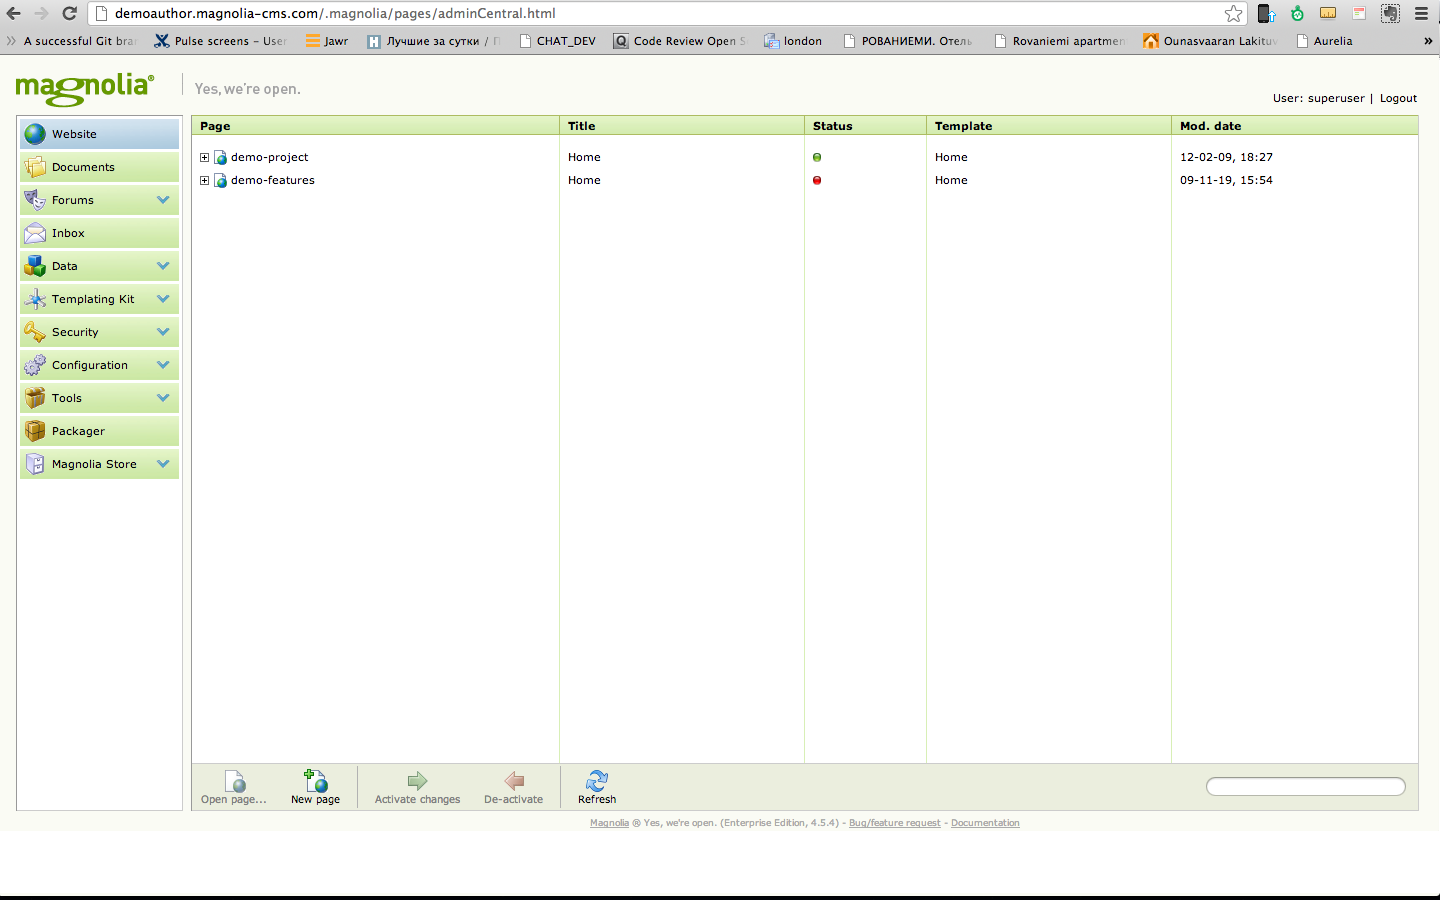
\includegraphics[width=\textwidth]{old_interface_magnolia.png}
  \caption[labelInTOC]{AdminCentral of Magnolia CMS 4.5}
  \label{fig: old_admin_central}
\end{center}
\end{figure}
However, this task is rather abstract and probably needs elaboration. Let us
observe the more specific assignments that could be spawned from it.

\section{Decoupling the Functionality of the Admin Interface}
Under decoupling here we mean separating the parts of interface into the logical
pieces that would describe themselves well and allow for adding the new ones
easilly. In order to provide the decoupling of current monolitic AdminCentral
interface there should be well-defined functionality units within the module.
Such units should cover a clear subset of the Magnolia CMS features just like an
application from the software suite. Thus, it makes sense to call the distinct
parts of a new interface \emph{applications} or simply \emph{apps}.

Developing the internal application framework is the key task in achieving the
final goal. The applications must be easy to build, integrate and style. In
spite of the distinct purposes and looks apps must have a common design.
Building an app should also require the least amount of boilerplate code. This
implies that a set of initial reusable components should be carefully designed
in order to reduce the boilerplate in the application code. It is also important
to develop the communication mechanism so that it is easy to send messages
between the apps.

\section{Improve Development Simplicity}
One of the biggest complexities in modern web application development is the
demand of mastering several programming languages and paradigms in order to
complete almost any project. Magnolia 5.0 targets reducing the amount of
technologies the app developer has to be familiar with (average knowledge of the
Java programming language should be enough). The client-server communication
should also be simplified as much as possible. As a consequence it would mean
abandoning the current Javascript based UI solution of AdminCentral and bringing
as much of its logic to server side as possible.
We will study how the task of building fully functioning web components can be
done without the involvement of client side programming by means of the Vaadin
application framework.

\section{Mobile First}
Mobile device platforms are becoming more and more popular nowadays. This is
mainly due to overcoming the technical barriers. The latest advancements in
technology progress gave users the hi-speed mobile Internet connection (3G, LTE)
the smartphones and tablets with computation power comparable to desktops. This
provides people with an opportunity to do the same tasks and jobs on mobile
devices as on the desktop computers. As a result - half of the world's web
traffic is mobile \cite{virtual_presence}.

There is a new trend called BYOD (Bring Your Own Device) - a movement or a
tendency of employees to use their own hardware at work. It has its roots in bad
user experience: people bring their devices to work because they want to
recreate the ease of use that they experience at home \cite{bkg_of_new_design}.
The main concept of BYOD is the requirement that the used software functions as
good on all major platforms and ideally - identically. Also it is hard to argue
with Borise's Kraft saying:
\emph{'If you compare today's bloated interfaces of enterprise software with the
fun-to-use, task-oriented apps on your iPhone you will immediately realize the
attraction of the latter'} \cite{mobile_first}.

Thus, supporting at least the major players in the mobile market (e.g. Apple iOs and
Google Android) is a must for Magnolia 5.0. This would involve the recognition
and support for touch events and gestures in order to give the editors the same
power as by the desktop version. 

\section{Performance and Scalability.}
The new interface must be scalable in terms of performance - visualization of
the tree structures with thousands of nodes must not be a problem. Data
management must avoid loading and keeping large datasets in memory and instead
rely onto lazy loading and caching mechanisms. For security reasons, the least
attainable amount of business logic should be exposed on the client side. 

UI scalability is also a requirement - in order to support extensions essential
Admin Interface has to support modular plugins a lot like modern mobile platforms 
support additional applications to be installed.

\section{CMS Deconstrution.}
The importance of a CMS admin interface was discussed before. It plays one of the
most significant roles in persuading the developers to use considered CMS. On the
other hand, even incredibly powerful CMS with poor user interface could make it
next to unusable.

Never the less, there is an indirect reason for struggling for delivering good
user experience. This reason is a lowering price and complexity of the other
systems' parts. The reduction is achieved by adopting the third-party products.
Indeed more and more utilities provided by a management suite can be separated
from it and be available as services. It is a common case that these sevices are
remote and even free. For instance, it makes little sense to develop the video
publishing and hosting facilities within the system - the team would rather use
YouTube or Vimeo. This could apply to various aspects of Content Management
System typical tasks (DropBox for file sharing, Google Analytics for analytics
etc).

This tendency could be defined by the term of \emph{Decomposition of Content
Managemet}. Even though this is not yet a rule of thumb for CMS developers - it
is already widely used. For instance Magnolia CMS uses CampaignMonitor for
e-mail campaigns and IntenseDebate for commenting.

It is quite obvious that such services would be available for any vendor of CMS
or any other type of management system. This fact increases the potential of the
high amount of comptetitors offering rich yet rather similar functionality.
It can be concluded that the biggest difference between the rivals is the
quality of integration with external services and the convenience of the
resulting composition.

Even though \emph{CMS Decomposition} is not the best approach for all the
development cases and a lot of the functionality has to be built from scratch -
an effort to provide the innovative and extensible user interface framework
could result into a significant advantage in the future \cite{cms_decomposition}.

\subsection{Summary}

All these requirements indicate that the resulting system is a very complex one.
Especially from the server side perspective but also from the client side (the
modern looking interface will inevitably need a lot of complex views and
transitions between them to be programmed). The client-server communication and
synchronization is also an important and non-trivial task to be accomplished.

In the following chapters we will observe how the key points described above
could be fulfilled by the combination of Magnolia, Vaadin and GWT. We will
discuss the reasons for choosing this stack of technologies and make an analysis
of the system architecture as well as go through the implementation details.

 \pagebreak